\documentclass[12pt]{article}

\usepackage{sbc-template}
\usepackage{graphicx,url}
\usepackage[brazil]{babel}
\usepackage[latin1]{inputenc}
\usepackage{lscape}
\usepackage{geometry}
\usepackage{float}
\usepackage{algorithm2e}
\usepackage{multicol}
\usepackage{amsmath}
\usepackage{amsfonts}
\usepackage{amssymb}
\usepackage{makeidx}
\usepackage{graphicx}
\usepackage{lmodern}
\usepackage{enumerate}
\usepackage{latexsym}
\usepackage{longtable}
\usepackage[all]{xy}
\usepackage{float}
\usepackage{lscape}
\usepackage{mathrsfs}
\usepackage{fancyhdr}
\usepackage{boxedminipage}
\usepackage{enumitem}


\sloppy

\title{Implementação do algoritmo k-NN}

\author{Marco Cezar Moreira de Mattos\inst{1}, Rômulo Manciola Meloca\inst{1}}

\address{DACOM -- Universidade Tecnológica Federal do Paraná (UTFPR)\\
  Caixa Postal 271 -- 87301-899 -- Campo Mourão -- PR -- Brazil
  \email{\{marco.cmm,rmeloca\}@gmail.com}
}

\begin{document}

	\maketitle

	\begin{resumo}
		Relata o procedimento tomado para implementar o algoritmo k-NN e os testes feitos com ele sobre um conjunto de dados.
	\end{resumo}

	\section{O algoritmo}\label{sec:algoritmo}
		
		O K-nearest neighbors (k-NN) é um algoritmo de classificação inteligente que avalia os k elementos mais similares ao elemento a que se deseja classificar e então rotula-o por meio de voto majoritário. É classificado como um algoritmo de aprendizagem supervisionada, de modo que exige um conjunto de treinamento já com as respostas de cada instância de treino.

		O k-NN pode calcular a proximidade de instâncias através da distância de Manhattan, distância euclidiana ou qualquer outra.

		Para analisar a taxa de acertos do algoritmo, observa-se na matriz de confusão quantas instâncias o k-NN classificou corretamente e quantas o algoritmo errou. Nesses casos, utiliza-se o o conjunto de treino, o conjunto de testes controlados para obter a taxa de acerto. Abaixo segue pseudo-código do algoritmo.

		\begin{algorithm}[H]
			\KwData{Conjunto de testes}
			\KwResult{Matriz de confusão}
			Inicializar matriz de confusão\;
			\For{all instâncias $\in$ Conjunto de treino}{
				distâncias = Nova lista\;
				\For{all instâncias $\in$ Conjunto de teste}{
					distância = Calcula a distância euclidiana\;
					distâncias.add(distância)\;
				}
				Ordenar(distâncias)\;
				Obter k menores distâncias\;
				Calcular a classe da instância mais votada\;
				Registrar resultado na matriz de confusão\;
			}
			\caption{Pseudo-código k-NN}
		\end{algorithm}

		Obviamente em um cenário real, ao ser empregado o algoritmo k-NN, não seria possível obter a matriz de confusão, dado que não se saberia de antemão, qual a real classificação de uma instância. Nesses casos, o retorno do algoritmo é a classe a que uma determinada instância pertence. Nestes termos, eliminaria-se o laço mais externo do algoritmo e as instruções referentes a matriz de confusão.

	\section{Implementação}\label{sec:implementacao}

		Optou-se por implementar o algoritmo k-NN na linguagem de programação Java. A seguir, diagrama de classes modelado para mapear o problema para o computador.

		\newgeometry{left=0cm,bottom=0cm,right=0cm,top=0cm}
		\begin{landscape}
		\centering
		\begin{figure}[p]
		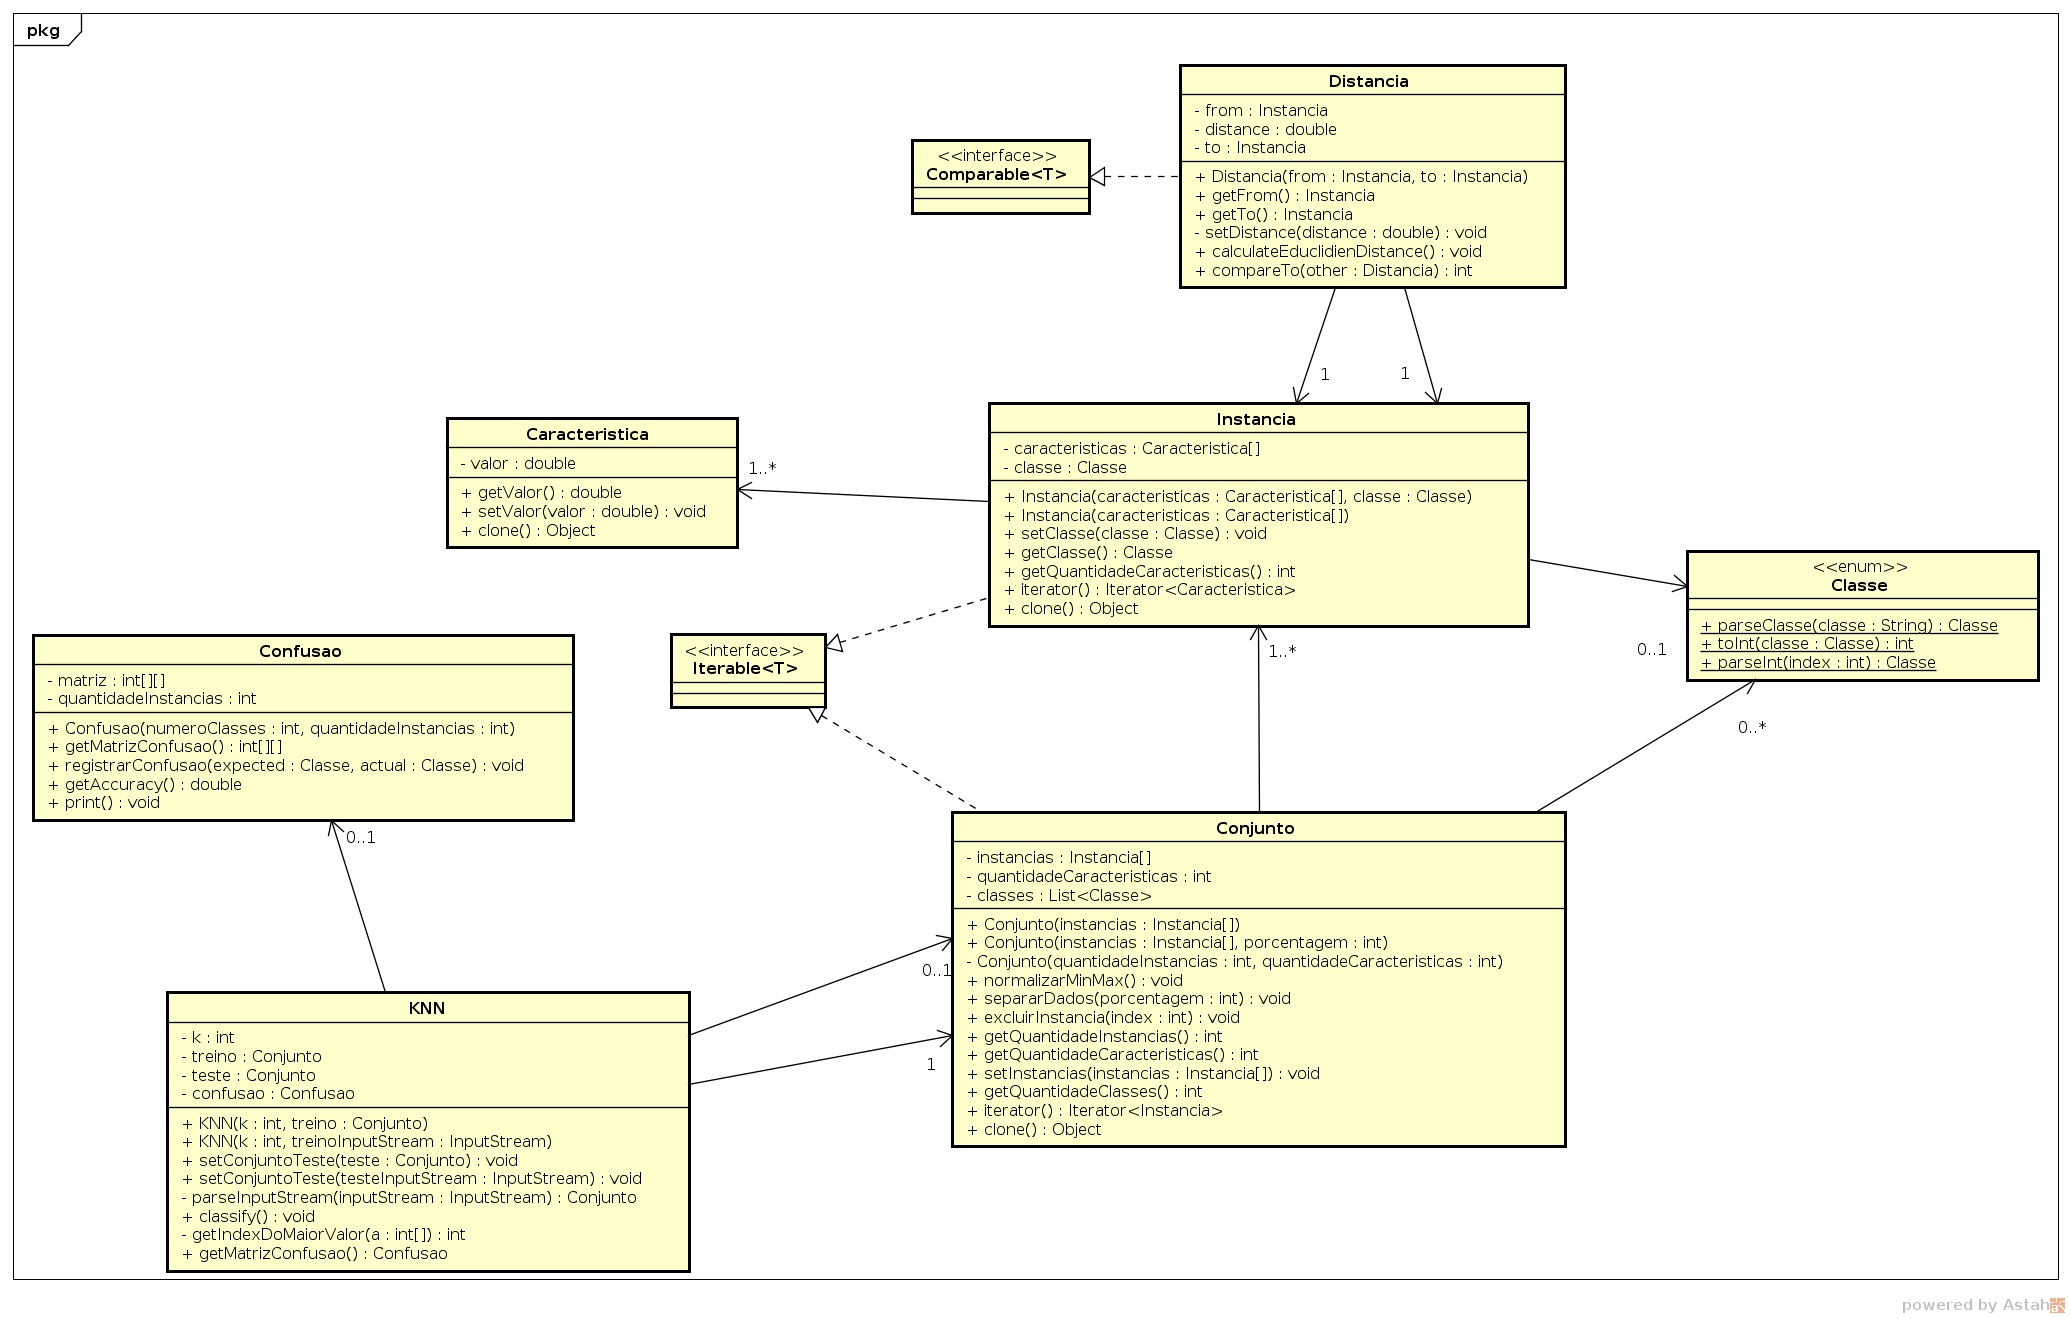
\includegraphics[width=1.4\textwidth]{classDiagram.png}
		\caption{Diagrama de Classes}
		\label{fig:classDiagram}
		\end{figure}
		\end{landscape}
		\restoregeometry

		Optou-se por utilizar a distância euclidiana como métrica, definida pela fórmula matemática a seguir:

		\noindent Sejam $x$ e $y$ vetores quaisquer de tamanho igual a $n$ e $x_{i}$ e $y_{i}$ respectivamente seus elementos,

		\quad\quad $Distancia = \sqrt{\sum_{i=1}^{n}(x_i - y_i)^2}$

		Para conjuntos de dados cujos elementos possuem alta discrepância entre si, faz-se necessário normalizar os dados. Optou-se por utilizar o Min-Max para normalizar os conjuntos de treino e teste. A técnica Min-Max define-se pelo que segue:

		\quad\quad $Valor' = (Valor - ValorMinimo)/(ValorMaximo - ValorMinimo)$

	\section{Testes}\label{sec:testes}

		Foram dados dois conjuntos com respostas. As instâncias dos conjuntos referiam-se aos meses do ano. No conjunto intitulado ``teste" constavam 1200 instâncias com 24 características cada. No conjunto intitulado ``treino" haviam 3600 instâncias também com 24 características cada. A fim de testar o algoritmo implementado, apropriou-se dos conjuntos de dados disponibilizados, bem como seguiu-se o que seus respectivos títulos sugeriam.

		Avaliou-se o impacto sobre a taxa de acerto quando:

		\begin{itemize}
			\item Variando-se o valor para $k$;
			\item Normalizando ou não os conjuntos;
			\item Selecionando partes aleatórias do conjunto de treinamento por meio de porcentagem.
		\end{itemize}

		Combinou-se os itens supracitados de variadas formas sob vários testes a fim de poder-se analisar o impacto das combinações possíveis para sa execução.
		
		Dado que os resultados obtidos não ultrapassaram a casa dos 60\% de acerto, observou-se que as taxas de acerto 
		mostraram-se consideravelmente baixas, todavia, não é possível inferir que o algoritmo, ou até mesmo a presente implementação foram ruins, uma vez que as características podem não ter sido bem escolhidas.

		Variando-se os valores para $k$ no conjunto dado, observou-se que as taxas diminuiam a medida que aumentava-se o valor para $k$.

		Normalizando-se o conjunto, observava-se que, ainda que $k$ fosse variado, as taxas sutilmente diminuiam (para espanto dos relatores) no conjunto dado.

		Selecionando-se partes aleatórias do conjunto, observou-se que as taxas de acerto igualmente variavam, atingindo valores bons (porém não superiores às taxas de 100\% das instâncias) e valores ruins.

		Assim, dado o fator estocástico não pôde-se avaliar com precisão o impacto direto para o algoritmo k-NN quanto a quantidade de instâncias consideradas no conjunto de treinamento e teste dados.

		Segue a baixo resultados obtidos pelo k-NN:

		Com 100\% das instâncias de treino.
			Usando MinMax para normalizar.
				k = 3: 0.5166;
				k = 5: 0.4991;
				k = 11: 0.4616;
			Sem normalizar.
				k = 3: 0.5866;
				k = 5: 0.5583;
				k = 11: 0.4658;
		Com 50\% das instâncias de treino.
			Usando MinMax para normalizar.
				k = 3: 0.6275;
				k = 5: 0.4791;
				k = 11: 0.4383;
			Sem normalizar.
				k = 3: 0.5483;
				k = 5: 0.5408;
				k = 11: 0.465;

		Com 25\% das instâncias de treino.
			Usando MinMax para normalizar.
				k = 3: 0.5075;
				k = 5: 0.53;
				k = 11: 0.4158;
			Sem normalizar.
				k = 3: 0.555;
				k = 5: 0.5191;
				k = 11: 0.4066;
				
	\section{Considerações Finais}\label{sec:consideracoesFinais}

		Incapacitados de saber se as características das instâncias dadas foram bem escolhidas, torna-se impossível discutir sobre as taxas de acerto obtidas.
		
		Aliado ao fator estocástico e ao conjunto de instâncias e características tomadas, torna-se igualmente impossível discutir se é melhor ou pior fornecer como entrada para o algoritmo k-NN menos instâncias.

		Levando-se em consideração que o escopo deste experimento não avaliou outros algoritmos para comparar as taxas de acerto, outras medidas de distância, técnicas de normalização ou ainda testes com outros conjuntos.

		Posto o espectro de possibilidades supracitado, cabe considerar, portanto, a implementação do algoritmo, que pelo fato de ser muito simples e ainda ser um algoritmo com aprendizagem supervisionada, o nota-se positivamente, especialmente quando o conjunto possui classes bem distintas, onde o algoritmo poderia ser preciso (uma vez que não adicionando-se valores probabilísticos nele).

		Considera-se ainda que variados valores para $k$ dependem do quão distantes encontram-se as classes no conjunto de treinamento.

		No escopo deste experimento, não foram identificados padrões que pudessem ser aqui relatados.

	\section{Referências}\label{sec:referencias}

		

\end{document}